\subsubsection[BDI]{BDI$^{\blacktriangle,\diamond}$}\label{fun:BDI}
Using cognitive modelling techniques for agent development enable autonomous behaviour and reasoning for automated problem solving.
This also allows the analysis of real world behaviour through simulations with agents.
Problems can hence be automatically solved through self-organised groups of agents and new knowledge can be drawn from such simulations.
The beliefs, desires and intentions (short: \emph{BDI}) model, is a widespread software model for developing intelligent agents situated in complex and dynamic environments.
There, the basic characteristics of an agents' mental state are expressed through beliefs, desires and intentions which are explained in more detail later in this section.
The BDI logic system is quite easy to implement in software agents and to some extent promises human-like reasoning behaviour.
Hence, it has been widely used in the field of artificial intelligence in computer science.
This section begins with the roots of the BDI model by mentioning the scientific papers that led to it.
It then continues with an explanation of practical reasoning after which the components of the BDI model are presented in greater detail.
% TODO if there is more to come, I will add it here. I still haven't made it through this text.

In 1987, Bratman~\cite{MICHAEL_PlansResource_1988} discussed the relationship between beliefs, desires, intentions and actions as well their roles in agent behaviours.
This can be seen as the introduction of the BDI model which was revised in 1991 by Rao and Georgeff~\cite{rao_modeling_1991}.
They formalised the model to a first order logic and treated beliefs, desires and intentions as three modal operators while giving intentions equal importance compared to beliefs and desires.
Rao and Georgeff then continued to apply this theoretical foundation to concrete BDI agents, applying them in an airline traffic management application~\cite{Rao_BDITheory_1995}.
Nowadays, BDI agents are deployed in high technology industrial areas such as fault diagnosis on space shuttles, but also in commercial fields and entertainment such as robot soccer games.

The BDI model has its roots in philosophy as found in Bratman's theory of practical reasoning~\cite{Sebastian_Hierarchical_2006}.
Practical reasoning involves two important processes: deciding what goals should be achieved, and how they should be achieved.
The former process is known as \emph{deliberation}, the latter as \emph{means-ends reasoning}~\cite{Gerhard_MultiSystem_1999}.
Means-ends reasoning is a method to make plans for achieving goals based on current states.
The idea of means-ends reasoning is to reduce the difference between the current state and the state where a goal is achieved.
For this purpose, the method is applied recursively.
When an agent is placed in an environment, it should autonomously decide what to do and how to do it.
In general, an agent could execute many different actions but maybe only a few of them would have a desired effect on the environment.
Various external properties can have influence on the feasibility of achieving the agent's goals\todo{\textbf{@yuansun1990}: this part confused me a bit. I don't think, \enquote{affairs} was the right word here. Please check if I still understood what you wanted to say.}.
The deliberation process filters what options are actually possible in the current state.
It then determines which of these options will become intentions.
For example, if you are thirsty and standing in a supermarket, then you might be faced with the decision to choose a drink.
There can be a lot of options like wine, beer, water, lemonade or juice.
However, picking up a bottle of wine or beer is not allowed in Germany for people under the age of 16. % Germany, sadly a proud nation of drunkards.
After collecting all the available options, you must choose and commit to some of them which become intentions next.
Subsequently, we need the mean-ends reasoning process to plan how to achieve these intentions.
If your intention is to buy a bottle of water, you may then plan to go to the shelf with water on it, reach for such a bottle, take it to the checkout counter and pay for it.
Finally, you have to execute this plan to buy the bottle of water.

The BDI model, as an applicable theory of practical reasoning, consists of three components which are beliefs, desires and intentions.
These are subsequently explained each.

Beliefs represent the informational part of the agent~\cite{Rao_BDITheory_1995} and are updated appropriately after each sensing action.
They may be implemented as a variable, a database, a set of logical expressions or some other data structure~\cite{Rao_BDITheory_1995}.
Beliefs model the agent's look at the world.
They can express information about the environment, other agents or the agent itself.
An agent may update its beliefs at any time.
Agents receive new information from the perception of the environment and the execution of intentions.
An agent can use sensors to perceive the environment and store their output as beliefs.
Beliefs are not the same concept as knowledge.
Knowledge is the realisation of a fact whereas a belief models \enquote{knowledge} which is believed by the agent.
Beliefs do not necessarily have to be true from a global perspective.
But from the agent's perspective, they are.
Hence, beliefs can be seen as local knowledge.
Likewise, beliefs can be global knowledge when they are true in a global sense.

Desires represent the motivational part of the agent~\cite{Rao_BDITheory_1995}.
In other words, desires represent objectives or situations that the agent would like to accomplish or bring about.
Desires can be but do not need to be achieved.
% Although similar, desires can be distinguished from goals.
Multiple desires can be inconsistent with each other and the agent does not need to know the means of achieving these desires.
They are inputs to the agent's deliberation process, which results in the agent choosing a subset of desires that are both consistent and achievable.
Such consistent and achievable desires are usually called \emph{goals}~\cite{Gerhard_MultiSystem_1999}.
For example, sleeping and working may be both one's desires, but they can not both be one's goals at the same time because they conflict with each other.

Intentions are desires or actions that an agent committed itself to achieve~\cite{Alejandro_LearnBDI_2004}.
Their meaning is stronger than that of desires.
Desires are merely wishes that may be achieved or may be not, but intentions are decided to be achieved to a reasonable extent.
Michael Wooldridge~\cite{Gerhard_MultiSystem_1999} concluded four functions of intentions in practical reasoning:
\begin{itemize}
  \item Intentions driving means-ends reasoning means that intentions have decisive influences on the actions which the agent will execute.
    Agents are expected to determine ways of achieving intentions.
  \item Intentions constrain future deliberation.
    This means that options which would be in conflict with an already chosen intention will not be considered.
  \item Intentions persist means that intentions will not be given up unless there is a rational reason to do so.
    This is important because if an agent immediately dropped its intentions without devoting resources to achieving them, it will never achieve anything~\cite{Gerhard_MultiSystem_1999}.
    Hence, intentions are committed desires which can not be easily abandoned.
    A reason to drop an intention nevertheless could be e.g. when an external event made the intention impossible or a lot more difficult to achieve.
  \item Intentions influence beliefs upon which future practical reasoning is based.
    This expresses that an intention is believed to be eventually achieved under \enquote{normal circumstances}.
    Practically, after deciding on an intention, the agent will add the intention as a belief.
    This allows the agent to plan for the future on the assumption that the intention will be achieved.
\end{itemize}
Intentions play an important role in the BDI model as they lead to actions and influence future beliefs and intention selection.

Beliefs, desires and intentions are the foundation of BDI agents.
Yet, further components are needed to build the connection between these three components and thereby implement BDI agents.
Naturally, the architecture of BDI agents differs in detail depending on their tasks.
However, they all share a core architecture which is depicted in \autoref{fig:bdi_architecture}.
Its components are explained in the following paragraphs.
\begin{figure}[htbp]
  \centering
  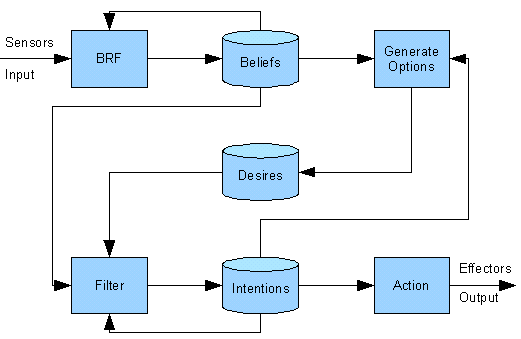
\includegraphics[width=\textwidth]{images/BDIAr}
  \caption{Brief BDI architecture~\cite{BDIA}}
  \label{fig:bdi_architecture}
\end{figure}

The sensors of a BDI agent perceive the environment and convert the perceptions to signals as inputs for the belief revision function (short: \emph{BRF}).
This function collects the external perceptions as well as the beliefs which are already stored in the beliefs.
It then processes the information and updates the beliefs accordingly.
The belief revision function prefers minimal change over modifying a lot and hence tries to preserve as much information as possible~\cite{Antje_SpatialBelief_2011}.
While processing the new and old information, the BRF will also solves inconsistencies, e.g.\ when an agent perceives information which contradicts a belief it has.

The belief set's data may be modelled as sentences, rules or some other manifestations.
In the \emph{AGM approach} (named after their proponents, Alchourrón, Gärdenfors, and Makinson)~\cite{alchourron_revision_1985}, an agent's beliefs are modeled by a deductively closed set of formulas called a \emph{belief set}~\cite{James_revise_2011}.
This approach is broadly used in belief revision research.
It makes several postulates for one revision operator which mapping each belief set and one sentence of beliefs to generate new beliefs.
Meanwhile, these postulates allow the belief revision process to retain as many previous beliefs as possible to reduce the amount of change.

The option generator reads the beliefs information and returns a list of options, which are current desires, into the desires set.
It determines the desires depending on the agent's current beliefs and current intentions.
The desires set contains desires, which are the possible courses of actions available to the agent.
These desires can be achievable or not.
The filter determines the agent's intentions depending on current beliefs, desires, and intentions.
It needs to reason about more situations than the functions in previous steps.
Desires will become more rational after filtering.

The intentions set stores the agent's current focus - the actions, which are going to be executed or committed to be executed at some point of time.
Once an intention is adopted, it should not be immediately dropped out because of the commitment.
But in some situations the intentions should be given up.
There are three commitment strategies proposed in Rao and Georgeff's work: blind, single minded and open minded.
A blindly committed agent is an agent who maintains his intentions until he believes that he has achieved them.
A single minded committed agent is an agent who maintains his intentions as long as he believes that they are still options.
An open minded committed agent is an agent who maintains his intentions as long as they are still goals~\cite{Roberto_BDIATL_2005}.
The action selection function determines the actions to perform depending on current intentions.
We would achieve nothing if we just have intentions instead of knowing how to do it.
Normally, there is a plan library of mappings between the intentions and actions.
The intentions go through the planner until the actions which mapped to the corresponding intentions are found.
Finally, a plan of how to achieve the intentions come out and the agent will execute these actions.

\autoref{tab:BDIC} summarises the BDI agent architecture as described by Michael Wooldridge~\cite{Gerhard_MultiSystem_1999}.
\begin{table}[!hbp]
  \label{tab:BDIC}
  \begin{tabularx}{\textwidth}{|l|p{5cm}| >{$}X<{$} |}
  \hline
  \textbf{Component} & \textbf{Meaning} & \textbf{Formalisation} \\
    \hline
    Belief set & Information about the current environment which the agent has & B \\
    \hline
    Belief revision function & determines a new set of beliefs depending on perceptual inputs and the agent's current beliefs & B \times P \to B\\
    \hline
    Options & determines desires depending on the agent's current beliefs and current intentions & B \times I \to D \\
    \hline
    Desires set & possible courses of actions available to the agent & D \\
    \hline
    Filter & determines the agent's intentions depending on current beliefs, desires, and intentions & B \times I \times D \to I \\
    \hline
    Intentions set & the agent's current focus & I \\
    \hline
    Action selection function & determines an action to perform depending on current intentions & I \to A  \\
    \hline
  \end{tabularx}
  \caption{Components of brief BDI agent architecture}
\end{table}

\autoref{tab:BDIC} shows the order of using the seven components of BDI architecture as well as giving the formulas for each function.
If we denote $Bel$ a set of all possible beliefs, $Des$ a set of all possible desires and $Int$ a set of all possible intentions.
Then an agent's state can be presented as $(B,D,I)$ with $B \subseteq Bel, D \subseteq  Des, I \subseteq  Int$~\cite{Gerhard_MultiSystem_1999}.
$P$ is a set of current perception which are obtained by the sensors of the agent.
We can understand the process of BDI agent working better through seeing this table.
Firstly, $B$ stores some beliefs which are read by BRF (belief revision function) while it getting the perception from the sensors.
After operating BRF, some of beliefs are removed, some are added, some are modified and so on.
So the new belief set $B$ built on basis of $P$ and original $B$.
Subsequently, Options use the new $B$ and current intentions set $I$ to determine the desires set $D$ and store it.
Moreover, the filter select intentions by referencing $B,D,I$, then the new intentions set comes out.
Finally, the action selection function makes a plan to execute actions to achieve $I$.

The process of $B \times P \to B$, $B \times I \to D$ and $B \times I \times D \to I$ belongs to deliberation.
They are deliberated in-depth gradually and the range of intentions are narrowed, especially the filter which should consider of all the datasets.
At last, the intentions are limited in particular ranges.
The plans will be made more effective and more targeted.
$I \to A $ can be treated as the process of means-ends reasoning, whose output is planning.
$B,D I$ are connected to function parts instead of connecting to each other directly, because they are treated as just databases and need rules or mechanism to help them execute actions.

With the increasing needs of intelligent agents, more and more applications base on BDI model are applied in our life.
For example, PRS~\cite{Ingrand_PRS_1992} and dMARS~\cite{Mark_dMARS_2004} are both BDI-based systems for the reaction control system of the NASA Space Shuttle Discovery.
Additionally, the air-traffic management system OASIS~\cite{Magnus_OASIS_1992} is well-known as a BDI-based agent.
The system architecture of OASIS is made up of one aircraft agent for each arriving aircraft and a number of global agents, including a sequencer, wind modeller coordinator and trajectory checker~\cite{Rao_BDITheory_1995}.
Furthermore, robot soccer which is designed using BDI model becomes very popular in universities.
We can feel that, BDI agents bring many profits to human beings, they make the life more convenient.
However, there is still space for development in this field.

Although the BDI model is developed during about 30 years, some obstacles are not overcome and some challenges are still there.
Most goals of BDI implementations are not explicit, and these goals should be reasoned out from current beliefs and intentions by agents themselves.
Besides, the BDI model contains three attributes: beliefs, desires and intentions.
In some situations, not all the three attributes are needed.
Sometimes, an agent collects the beliefs and jumps to intentions directly without desires.
However, for some distributed multi-agents, just three attributes are not sufficient to execute the actions.
Furthermore, the agents in the multi-agents system do not have an explicit mechanism for interaction and integration among them.
When an increasing number of agents join the system, the interaction with each agent will be more and more difficult.
As an intelligent agent, the BDI agent do not have a good ability to learn from the past behavior or other agents’ behavior.
So that the rate of development will not be high, lacking mechanisms to learn from others.
However, BDI model has its own advantages.
Beliefs, desires and intentions are similar to the mental activities of human beings.
Therefore, it is not easy to construct the logics or mechanisms for it.
With the wildly used of computers and mobile devices, the situation of multi-agent interaction will be better.
As many computer languages and logic languages are grasped by more people, the BDI agent will bring human beings more surprises.

Beliefs, desires and intentions were introduced in this section.
The BDI agent belongs to the kind of intelligent agents which are autonomous, computational entities.
The BDI agent executes actions on the basis of BDI model that containing three main attributes which have close relationship between each other.
The brief BDI agent architecture is a clear description of process of how BDI agents work.
They follows the practical reasoning theory.
Different BDI implementations show different architectures, but the in core of these agents are still notions of beliefs, desires and intentions.

With an increasing number of BDI applications coming into the human life, more challenges come up too.
One of such challenges, which is the correctness of agents' behaviour, is described in the ~\autoref{fun:formal_methods} that follows.
Also, in the following section after introducing all the required logical operations and methods, a sample structure of an abstract BDI interpreter will be given, which also continues the topic discussed in this section.
